\documentclass{article}
\usepackage{ae,aecompl}
\usepackage{todonotes}
\usepackage{chngcntr}
\usepackage{tikz-cd}
\usepackage{graphicx}
\graphicspath{ {./images/}}
\usepackage[all,cmtip]{xy}
\usepackage{amsmath, amscd}
\usepackage{amsthm}
\usepackage{amssymb}
\usepackage{amsfonts}
\usepackage{bm}
\usepackage{qsymbols}
\usepackage{latexsym}
\usepackage{mathrsfs}
\usepackage{mathtools}
\usepackage{cite}
\usepackage{color}
\usepackage{url}
\usepackage{enumerate}
\usepackage{verbatim}
\usepackage[draft=false, colorlinks=true]{hyperref}
\usepackage{pdfpages}
\usepackage[margin=1.2in]{geometry}
\usepackage{IEEEtrantools}

\usepackage{fancyhdr}


\usepackage[nameinlink]{cleveref}


\DeclareMathOperator*{\ac}{accept}
\DeclareMathOperator*{\amax}{argmax}
\DeclareMathOperator*{\amin}{argmin}
\DeclareMathOperator*{\Aut}{Aut}
\newcommand {\al}{{\alpha}}
\newcommand {\abs}[1]{{\left\lvert#1\right\rvert}}
\newcommand {\A}{{\mathcal{A}}}
\newcommand {\AM}{{\mathrm{AM}}}
\newcommand {\AMp}{{\AM_{p}^{X}\!(\Ri_\w)}}
\newcommand {\B}{{\mathcal{B}}}
\DeclareMathOperator*{\Be}{Bern}
\newcommand {\Br}{{\dot{B}}}
\newcommand {\Ba}{{\mathfrak{B}}}
\newcommand {\C}{{\mathbb C}}
\newcommand {\ce}{\mathrm{c}}
\newcommand {\Ce}{\mathrm{C}}
\newcommand {\Cc}{\mathrm{C_{c}}}
\newcommand {\Ccinf}{\mathrm{C_{c}^{\infty}}}
\DeclareMathOperator{\cov}{Cov}
\DeclareMathOperator{\DEV}{DEV}
\newcommand {\Di}{{\mathbb D}}
\newcommand {\dom}{\mathrm{dom}}
\newcommand{\dist}{\stackrel{\mathrm{dist}}{=}}
\newcommand {\ud}{\mathrm{d}}
\newcommand {\ue}{\mathrm{e}}
\newcommand {\eps}{\varepsilon}
\newcommand {\veps}{\varepsilon}
\newcommand {\vrho}{{\varrho}}
\newcommand {\E}{{\mathbb{E}}}
\newcommand {\Ec}{{\mathcal{E}}}
\newcommand {\Ell}{L}
\newcommand {\Ellp}{{L_{p}[0,1]}}
\newcommand {\Ellpprime}{{L_{p'}([0,1])}}
\newcommand {\Ellq}{{L_{q}([0,1])}}
\newcommand {\Ellqprime}{{L_{q'}([0,1])}}
\newcommand {\Ellr}{L^{r}}
\newcommand {\Ellone}{{L_{1}([0,1])}}
\newcommand{\Elltwo}{{L_{2}([0,1])}}
\newcommand{\Ellinfty}{L^{\infty}}
\newcommand{\Ellinftyc}{L_{\mathrm{c}}^{\infty}}
\newcommand{\exb}[1]{\exp\left\{#1\right\}}
\DeclareMathOperator*{\Ext}{Ext}
\newcommand{\F}{{\mathcal{F}}}
\newcommand{\Fe}{{\mathbb{F}}}
\newcommand{\G}{{\mathcal{G}}}
\newcommand{\HF}{\mathcal{H}_{\text{FIO}}^{1}(\Rd)}
\newcommand{\Hr}{H}
\newcommand{\HT}{\mathcal{H}}
\newcommand{\ui}{\mathrm{i}}
\newcommand{\I}{{I}}
\newcommand{\J}{{\mathcal{J}}}
\newcommand{\id}{{\mathrm{id}}}
\newcommand{\iid}{\stackrel{\mathclap{\normalfont\mbox{iid}}}{\sim}}
\newcommand{\im}{{\text{im }}}
\newcommand{\ind}{{\perp\!\!\!\perp}}
\DeclareMathOperator*{\Int}{int}
\newcommand{\intx}{{\overline{\int_{X}}}}
\newcommand{\inte}{{\overline{\int_{\E}}}}
\newcommand{\la}{\lambda}
\newcommand{\rb}{\rangle}
\newcommand{\lb}{{\langle}}
\newcommand{\La}{\Lambda}
\newcommand{\calL}{{\mathcal{L}}}
\newcommand{\lp}{{\mathcal{L}}^{p}}
\newcommand{\lpo}{{\overline{\mathcal{L}}^{p}\!}}
\newcommand{\Lpo}{{\overline{\Ell}^{p}\!}}
\newcommand{\M}{{\mathbf{M}}}
\newcommand{\Ma}{{\mathcal{M}}}
\newcommand{\N}{{{\mathbb N}}}
\newcommand{\Na}{{{\mathcal{N}}}}
\newcommand{\norm}[1]{\left\|#1\right\|}
\newcommand{\normm}[1]{{\left\vert\kern-0.25ex\left\vert\kern-0.25ex\left\vert #1 
    \right\vert\kern-0.25ex\right\vert\kern-0.25ex\right\vert}}
\newcommand{\Om}{{{\Omega}}}
\newcommand{\one}{{{\bf 1}}}
\newcommand{\pic}{\text{Pic }}
\newcommand{\ph}{{\varphi}}
\newcommand{\Pa}{{\mathbb{P}}}
\newcommand{\Po}{{\mathcal{P}}}
\newcommand{\Q}{{\mathbb{Q}}}
\newcommand{\R}{{\mathbb R}}
\newcommand{\Rd}{{\mathbb{R}^{d}}}
\DeclareMathOperator{\rej}{reject }
\newcommand{\Rn}{{\mathbb{R}^{n}}}
\newcommand{\cR}{{\mathcal{R}}}
\newcommand{\Rad}{{\mathrm{Rad}}}
\newcommand{\ran}{{\mathrm{ran}}}
\newcommand{\Ri}{{\mathrm{R}}}
\newcommand{\supp}{{\mathrm{supp}}}
\newcommand{\Se}{\mathrm{S}}
\newcommand{\Sp}{S^{*}(\Rn)}
\newcommand{\St}{{\mathrm{St}}}
\newcommand{\Sw}{\mathcal{S}}
\newcommand{\T}{{\mathcal{T}}}
\newcommand{\ta}{{\theta}}
\newcommand{\Ta}{{\Theta}}
\newcommand{\topp}{\stackrel{p}{\to}}
\newcommand{\todd}{\stackrel{d}{\to}}
\newcommand{\toL}[1]{\stackrel{L^{#1}}{\to}} 
\newcommand{\toas}{\stackrel{a.s.}{\to}}
\DeclareMathOperator{\V}{Var}
\newcommand {\w}{{\omega}}
\newcommand {\W}{{\mathrm{W}}}
\newcommand {\Wnp}{\text{$\mathrm{W}$\textsuperscript{$n,\!p$}}}
\newcommand {\Wnpeq}{\text{$\mathrm{W}$\textsuperscript{$n\!,\!p$}}}
\newcommand {\Wonep}{\text{$\mathrm{W}$\textsuperscript{$1,\!p$}}}
\newcommand {\Wonepeq}{\text{$\mathrm{W}$\textsuperscript{$1\!,\!p$}}}
\newcommand {\X}{{\mathcal{X}}}
\newcommand {\Z}{{{\mathbb Z}}}
\newcommand {\Za}{{\mathcal{Z}}}
\newcommand {\Zd}{{\Z[\sqrt{d}]}}
\newcommand {\vanish}[1]{\relax}

\newcommand {\wh}{\widehat}
\newcommand {\wt}{\widetilde}
\newcommand {\red}{\color{red}}

% Distributions
\newcommand{\normal}{\mathsf{N}}
\newcommand{\poi}{\mathsf{Poisson}}
\newcommand{\bern}{\mathsf{Bernoulli}}
\newcommand{\bin}{\mathsf{Binomal}}
\newcommand{\multi}{\mathsf{Multinomial}}
\newcommand{\Exp}{\mathsf{Exp}}



% put your command and environment definitions here




% some theorem environments
% remove "[theorem]" if you do not want them to use the same number sequence


  \newtheorem{thrm}{Theorem}
  \newtheorem{lemma}{Lemma}
  \newtheorem{prop}{Proposition}
  \newtheorem{cor}{Corollary}

  \newtheorem{conj}{Conjecture}
  \renewcommand{\theconj}{\Alph{conj}}  % numbered A, B, C etc

  \theoremstyle{definition}
  \newtheorem{defn}{Definition}
  \newtheorem{ex}{Example}
  \newtheorem{exs}{Examples}
  \newtheorem{question}{Question}
  \newtheorem{remark}{Remark}
  \newtheorem{notn}{Notation}
  \newtheorem{exer}{Exercise}

\DeclareMathOperator*{\bias}{Bias}


\title{STATS305A - Lecture 12}
\author{John Duchi\\ Scribed by Michael Howes}
\date{10/28/21}

\pagestyle{fancy}
\fancyhf{}
\rhead{STATS305A - Lecture 12}
\lhead{10/28/21}
\rfoot{Page \thepage}

\begin{document}
\maketitle
\tableofcontents
\section{Announcements}
\begin{itemize}
    \item Etude 2 due today 5pm.
    \item No class next Tuesday.
\end{itemize}
\section{Model Selection and prediction}
\subsection{Motivation}
Up to this point we've treated the model $Y=X\beta + \eps$ as ``god-given''. This is a bit inaccurate. In real life we will typically have data and no model and have to figure it out and select a model. When selecting a model we have two desiderata:
\begin{itemize}
    \item Identify important features that are relating $x$ to our response $y$.
    \item Pure predictive accuracy: how well can we predict $y$ from $x$?
\end{itemize}
These two are intertwinned. We don't always have to choose one over the other.
\subsection{In sample and out of sample risk}
Suppose we are in a setting where $y = f(x)+\eps$ and $\E[\eps|x]=0$. This is equivalent to having $f(x) = \E[Y|X=x]$ since if $\eps = y-f(x)$, then \[\E[\eps|x] = \E[y|x] - f(x).\]
Thus $\E[\eps|x]=0$ if and only if $f(x) = \E[y|x]$. Define $\sigma^2(x) = \E[\eps^2|x]$ which is the conditional variance of $\eps$. 

Our goal is to fit a predictor $\wh{f}$ using a sample $\{(x_i,y_i)\}_{i=1}^n$. Note that if we think of the sample of $\{(x_i,y_i)\}_{i=1}^n$ as random, then the predictor $\wh{f}$ is random (like how $\wh{\beta}$ is random in the linear model). Thus we can take the expectation of quantities involving $\wh{f}$ over all samples $\{(x_i,y_i)\}_{i=1}^n$. This idea will be used many times over the course of this lecture. 
\begin{defn}
    If we have a predictor $\wh{f}$ of a model $y = f(x)+\eps$, then we define the \emph{in-sample (MSE) risk} of $\wh{f}$ to be 
    \[R_{in}(\wh{f}) = \E\left[\frac{1}{n}\sum_{i=1}^n (\wh{f}(x_i)-f(x_i))^2\right], \]
    where the above expectation is taken over all samples $\{(x_i,y_i)\}_{i=1}^n$ with $x_i$ fixed. (That is we fix $x$ and calculate $\wh{f}$ using different samples $(x,y)$, we then calculate the quantity $\frac{1}{n}\sum_{i=1}^n (\wh{f}(x_i)-f(x_i))^2$ and take the expectation over all samples $(x,y)$.)
\end{defn}
\begin{aside}
    Sometimes the in-sample risk is called the $L^2(P_n)$ risk. This is because $R_{in}$ is the expectation of the squared $L^2$ norm error of $\wh{f}-f$ with respect to the distribution
    \[P_n = \frac{1}{n}\sum_{i=1}^n \one_{x_i}.\]
\end{aside}
\begin{defn}
    Sometimes the insample risk is defined with respect to a fresh sample $\{Y_i^*\}_{i=1}^n$ where 
    \[Y_i^* = \text{ a new sample of } Y_i = f(x_i) + \eps_i^*, \]
    where $\eps_i^*$ is an independent copy of $\eps_i$. We then define
    \[R_{in}^*(\wh{f}) = \E\left[\frac{1}{n}\sum_{i=1}^n \left(Y_i^*-\wh{f}(x_i)\right)^2\right], \]
    where here the expectation is over both $Y_1,\ldots, Y_n$ (used to calculate $\wh{f}$) and over $Y_1^*,\ldots, Y_n^*$ (used to calculate $(Y_i^*-\wh{f}(x_i))^2$).
\end{defn}
Note that 
\begin{align*}
    R^*_{in}(\wh{f}) &= \E\left[\frac{1}{n} \sum_{i=1}^n (Y_i^*-\wh{f}(x_i))^2\right]\\
    &=\E\left[\frac{1}{n} \sum_{i=1}^n (Y_i^*-f(x_i))^2\right]+\E\left[\frac{1}{n}\sum_{i=1}^n (\wh{f}(x_i)-f(x_i))^2\right]\\
    &=\frac{1}{n}\sum_{i=1}^n \sigma^2(x_i)+R_{in}(\wh{f}).
\end{align*}
We call $\frac{1}{n}\sum_{i=1}^n \sigma^2(x_i)$ the irreducible error. 

Now suppose that we have a function $g:\X \to \R$ where $\X$ is the space $X$ lives in. Note that $g$ is different to $\wh{f}$. The predictor $\wh{f}$ is something that depends on the sample $(x,y)$ used to fit $\wh{f}$. The function $g$ is simply a function. It is a way of taking an $X$ and producing a number. With this in mind we have our next definition.
\begin{defn}
    Given a function $g : \X \to \R$, the \emph{out of sample (MSE) risk} of $g$ is
    \[R_{out}(g) = \E[(Y-g(X))^2] = \int_\X \E[(Y-g(x))^2|X=x]p(x)dx. \]
    Here the expectation is over both $Y$ and $X$ (hence out of sample - we are allowing $X$ to change).
\end{defn}
Note that 
\begin{align*}
    R_{out}(g) &= \E\left[(Y-f(X)+f(X)+g(X))^2\right]\\
&=\E\left[(Y-f(X))^2\right]+\E[(f(X)-g(X))^2]+2\E\left[(Y-f(X))(f(X)-g(X))\right]\\
&=\E[\sigma^2(X)]+\E[(f(X)-g(X))^2].
\end{align*}
We again call $\E[\sigma^2(X)]$ the irreducible error and we could call $\E[(f(X)-g(X))^2]$ the ``error in mean prediction'' (this last term is just a term John used - he said that there isn't really a term in literature for $\E[(f(X)-g(X)^2)]$).

In the out of sample risk we average over all the $X$'s we could possible draw. In the in sample we fix the value $x_i$ and average over all possible $y_i$. Note that if our data is i.i.d., then 
\[R_{out}(g) = \E[(g(X_{n+1})-Y_{n+1})^2]. \]

 The quantity $R_{out}(\wh{f})$ is a number but it is random since it depends on the sample $(x_i,y_i)_{i=1}^n$ used to fit $\wh{f}$ and the sample $(x_i,y_i)_{i=1}^n$ is random. Thus $\E[R_{out}(\wh{f})]$ is our expected out of sample risk over all samples used to fit $\wh{f}$.
 
 \subsection{Bias/variance decomposition}
 Let $\wh{f}$ be any estimator of $f$. For any $x \in \X$ we can write
 \begin{align*}
     \E[(\wh{f}(x)-f(x))^2] &= \E\left[\left(\wh{f}(x)-\E[\wh{f}(x)]+\E[\wh{f}(x)]-f(x)\right)^2\right]\\
     &= \E[\left(\wh{f}(x)-\E[\wh{f}(x)]\right)^2]+\left(\E[\wh{f}(x)]-f(x)\right)^2\\
     &= \V(\wh{f}(x))+\bias(\wh{f}(x))^2,
 \end{align*}
where, as in $R_{in}(\wh{f})$, the above expectation is taken with respect to the samples used to fit $\wh{f}$. Thus we have
\[R_{in}(\wh{f})= \frac{1}{n}\sum_{i=1}^n \left(\bias(\wh{f}(x_i))^2+\V(\wh{f}(x_i))\right),\]
and 
\begin{align*}
    \E[R_{out}(\wh{f})]&= \E[\sigma^2(X)]+\E[\bias(\wh{f}(X))^2]+\E[\V(\wh{f}(X))]\\
    &= \text{irreducible error }+\text{ expected bias squared }+\text{ expected variance}. 
\end{align*}
This decomposition means that in practice we often see the following curve when we plot error against model complexity. The error initally goes down as complexity increases but then increases. This is because intially the model has high bias when the model is simple but once the model is very complicated it has high variance.

\begin{center}
    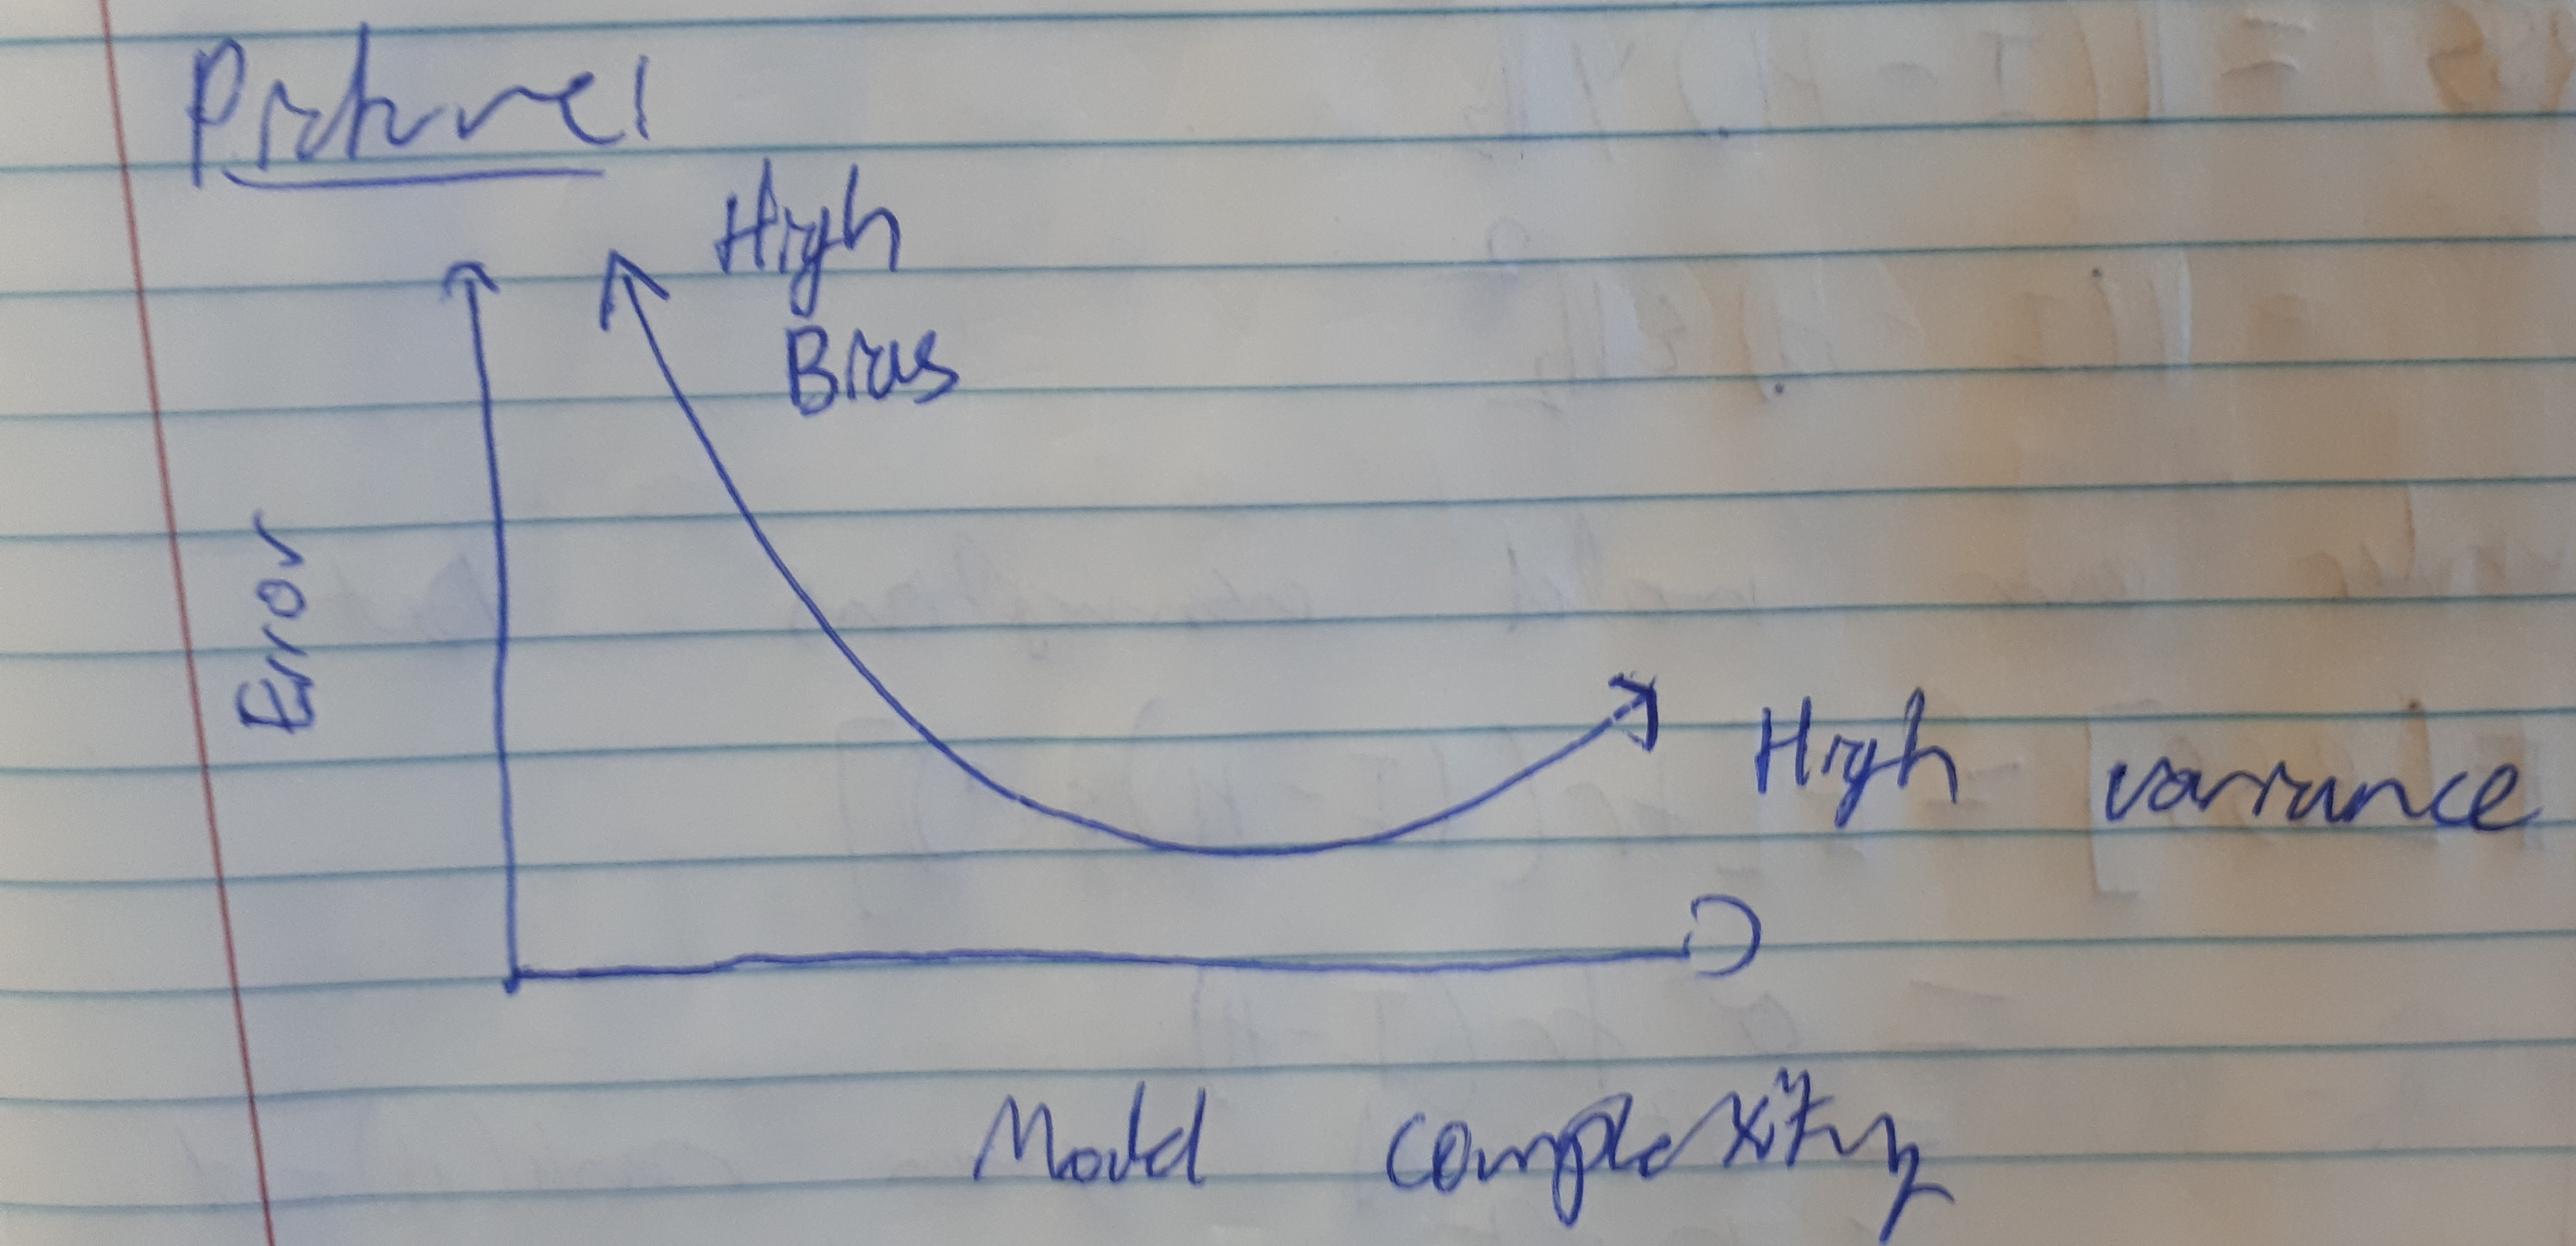
\includegraphics[width = \textwidth/2]{10_28_P01.jpg}
\end{center}

Although one word of warning: We sometimes don't know how to properly measure model complexity. This means that when we use a proxy for model complexity we might not see the above picture. This is sometimes the case with machine learning algorithms where the error continues to go down even as the number of parameters is getting very very high. The complexity of the model may not be as high as the number of parameters suggests.

\subsection{Comparing models}
The above analysis gives us the idea that we should choose a model that trades optimally between bias and variance. Unfortunately we can't do this exactly since we can only approximate the bias and variance of a model. We thus will have to estimate the prediction error. We can then use this estimate to choose a model. There is a challenge though, the natural quantity
\[\frac{1}{n}RSS = \frac{1}{n}\sum_{i=1}^n \left(Y_i  \wh{Y}_i\right)^2 = \frac{1}{n}\sum_{i=1}^n \left(Y_i-\wh{f}(x_i)\right)^2, \]
is biased downwards since we chose $\wh{f}$ to minimize RSS. Thus $\frac{1}{n}RSS$ will tend to  be smaller than $R_{in}^*$ since in $R_{in}^*$ we have a new independent sample of $Y$'s.

\begin{ex}
    Consider for concreteness the linear model $Y=X\beta + \eps$ where $\eps \sim (0, \sigma^2I_n)$ and $X$ is full rank with $\text{rank}(X) = d$. Let $H=X(X^TX)^{-1}X^T$, we know that \[RSS = \norm{(I-H)Y}_2^2 = \norm{(I-H)\eps}_2^2.\] Thus we have 
    \begin{align*}
        \E[RSS] &= \E[\tr((I-H)\eps\eps^T)]\\
        &=\sigma^2\tr(I-H)\\
        &=\sigma^2(n-d)\\
        &< \sigma^2 n.
    \end{align*}
    Thus $\E\left[\frac{1}{n}RSS\right] = \frac{n-d}{n}\sigma^2 < \sigma^2$ which is a problem since the irreducible error is $\sigma^2$ so we will always have $R_{in}^* \ge \sigma^2$.
\end{ex}
There are two approaches to overcome this issue:
\begin{enumerate}
    \item Penalized risk estimates.
    \item Validation.
\end{enumerate}
We will discuss the first approach today.

\subsection{Estimating risk}
How do we estimate the risk of a model? Let's think about the sum of square errors. Note that
\begin{align*}
    \E\left[\left(Y_i-\wh{Y}_i\right)^2\right]&=\E\left[\left(Y_i-f(x_i)+f(x_i)-\wh{Y}_i\right)^2\right]\\
    &=\sigma_i^2+2\E\left[(Y_i-f(x_i))(f(x_i)-\wh{Y}_i)\right]+\E\left[\left(f(x_i)-\wh{f}(x_i)\right)^2\right]\\
    &=\sigma_i^2+\E\left[(f(x_i)-\wh{f}(x_i))^2\right]-2\cov(Y_i,\wh{Y}_i)
\end{align*}
The last equality holds because $f(x_i) = \E[Y_i]$ and so for any constant $c_i$
\[\E\left[(Y_i-f(x_i))(\wh{Y}_i-c_i)\right] = \E\left[(Y_i-f(x_i))(\wh{Y}_i-\E[\wh{Y}_i])\right] =\cov(Y_i,\wh{Y}_i).\]
Thus we have 
\begin{align*}
    \E[RSS] &= \E\left[\sum_{i=1}^n (Y_i-\wh{Y}_i)^2\right]\\
    &=\sum_{i=1}^n \sigma^2_i + \sum_{i=1}^n\E\left[(f(x_i)-\wh{f}(x_i))^2\right]-2\cov(Y,\wh{Y}) \\
    &=\sum_{i=1}^n \sigma^2_i + nR_{in}(\wh{f})-2\cov(Y,\wh{Y}).
\end{align*}
Equivalently,
\begin{align*}
    R^*_{in}(\wh{f})&=R_{in}(\wh{f})+\frac{1}{n}\sum_{i=1}^n \sigma_i^2\\
    &= \frac{1}{n}\E[RSS]+\frac{2}{n}\cov(Y,\wh{Y}).
\end{align*}
The quantity $\cov(Y,\wh{Y})$ is called the ``effective degrees of freedom''. The upshot of these calculations is that if we can estimate $\frac{2}{n}\cov(Y,\wh{Y})$, then we can estimate the in-sample risk of $\wh{f}$. 

\begin{ex}
    Let's calculate the $\cov(Y,\wh{Y})$ in some special cases. Suppose we have a ``true'' linear model $Y=X\beta + \eps$ with $\eps \sim (0,\sigma^2I_n)$ and we fit $\wh{Y} = HY$. Then
    \begin{align*}
        \cov(Y,\wh{Y}) &= \cov(\eps, H\eps)\\
        &=\E[\eps^TH\eps]\\
        &=\sigma^2\tr(H)\\
        &=\sigma^2d,
    \end{align*}
    if $H$ has rank $d$. Suppose know that we don't know that $Y$ comes from a linear model but we have the more general model $Y_i = f(x_i)+\eps_i$. Suppose we still fit $\wh{f}(x) = x^T\wh{\beta}$ where $\wh{\beta} = (X^TX)^{-1}X^TY$. We then still have $\wh{Y} =HY$ and so
    \begin{align*}
        \cov(Y,\wh{Y}) &= \cov(\eps, HY)\\
        &=\cov(\eps, H[f(x_i)+\eps_i]_{i=1}^n)\\
        &=\cov(\eps, H\eps)\\
        &= \sum_{i=1}^n \sigma_i^2 H_{ii},
    \end{align*} 
    where $\sigma_i^2 = \V(Y_i) = \V(\eps_i)$. If we have homoscedastic noise, then $\sigma_i^2 =\sigma$ for all $i$ and 
    \[\cov(Y,\wh{Y}) = \sigma^2d, \]
    where again $d$ is the rank of $H$. These two examples give motivation for calling $\cov(Y,\wh{Y})$ the effective degrees of freedom.
\end{ex}
\begin{defn}
    \emph{Mallow's $C_p$ statistic} is the statistic.
    \[C_p := \frac{1}{n}RSS + 2\frac{\sigma^2}{n}\rank(X)=\frac{1}{n}RSS+2\frac{\sigma^2}{n}p, \]
    where $p=\rank(X)$. 
\end{defn}
\begin{defn}
    \emph{Mallow's method} is the following.
    \begin{itemize}
        \item Given a number of possible models, calculate $C_p$ for each model.
        \item Choose the model that minimizes $C_p$
    \end{itemize} 
\end{defn}
Unfortunately we do not know $\sigma^2$ and so to use Mallow's method we have to estimate $\sigma^2$. Some options are
\begin{enumerate}
    \item If we have a pair $\left(Y_i^{(1)}, Y_i^{(2)}\right)$ for each $x_i$, then $\E\left[\left(Y_i^{(1)}-Y_i^{(2)}\right)^2\right] =2\sigma$ and so we can use
    \[\wh{\sigma}^2 = \frac{1}{2n}\sum_{i=1}^n \left(Y_i^{(1)}-Y_i^{(2)}\right)^2. \]
    \item If we do not have paired data, then we can find $x$'s that are close to each other. We can then pair these $x$'s and use the above estimator.
    \item We can also use the most complicated model to estimate $\sigma^2$. Suppose that we have $Z \in \R^{n \times q}$ where $q$ is very big. Then we can define 
    \[\wh{\gamma} = (Z^TZ)^{-1}Z^TY \in \R^q, \]
    and use the estimator
    \[\wh{\sigma}^2 = \frac{1}{n-q} \sum_{i=1}^n (Y_i-Z_i^T\wh{\gamma})^2.\]  
\end{enumerate}
\end{document}